\documentclass[12pt,a4paper]{report}     % font size= 12,paper size= a4, document type= report 
\usepackage{graphics}
\usepackage[font=small,labelfont=bf]{caption}
\usepackage{fancybox}		% For formatting of cover page5
\usepackage{amsmath}    	% For  mathematical formulae
\usepackage{amssymb}
\usepackage{setspace}		% For adjusting line spacing 
\usepackage{pdfpages}
\usepackage{hyperref}                     % pacakage for 
\usepackage{fancyhdr}                     % pacakage for including header and footer 
%\usepackage{times}                        % package for font type
\usepackage[left=1in,right=1in,top=1in,bottom=0.8in]{geometry} %
\usepackage{url}
\usepackage{rotating}
\usepackage{array}
\usepackage{enumitem}
%\usepackage{bbding}
\usepackage{amsfonts}
\usepackage{float} 
\usepackage{listings}
\makeatletter
\def\@makechapterhead#1{%
  \vspace*{5\p@}%
  {\parindent \z@ \raggedright \normalfont
    \ifnum \c@secnumdepth >\m@ne
       \LARGE\bfseries \space \thechapter. \space
    \interlinepenalty\@M
    \LARGE \bfseries #1\par\nobreak
    \vskip 10\p@
  }}
  \makeatother
\begin{document}
\newpage
\pagestyle{plain}
\pagestyle{empty}
\pagestyle{fancy}							%display header, footer
\renewcommand{\headrulewidth}{0pt}
%\pagenumbering{arabic}						%display page numbers in arabic								 %set header to left	

%\fancyfoot[LO]{\textit{P:F-SMR-UG/08/R0}}			%set footer to left
\fancypagestyle{plain}{}

 %\thispagestyle{empty}
	\pagenumbering{gobble}
	\thisfancyput(-0.0in,-10.0in){%
	%\thisfancypage{%
%\setlength{\fboxrule}{1pt}\doublebox}{} 
\setlength{\unitlength}{1in}\framebox(6.7,10.2)}
\begin{center}
      
      \begin{center} {A} \end{center}
      \vspace{0.2 in}
      { PRELIMINARY PROJECT REPORT}
      \vspace{0.2 in}\\
       ON
			\end{center}
	\begin{center}
	    \vspace{0.1 in}
		\textbf{\large  Constellation - an MLOps platform  } % Give Your Seminar Title
		\vspace{0.2 in}
	\end{center}
     \vspace{0.2 in}
		\begin{center}
	    SUBMITTED TO THE SAVITRIBAI PHULE PUNE UNIVERSITY, PUNE \\
	    IN PARTIAL FULFILLMENT OF THE REQUIREMENTS\\
	    FOR THE AWARD OF THE DEGREE OF
	\end{center}
	\vspace{0.1 in}
	
	\begin{center}
	   {BACHELOR OF ENGINEERING}\\
	    \begin{small}{ INFORMATION TECHNOLOGY}
\end{small}	\end{center}
	\vspace{0.1 in}
	
	\begin{center}
	   \textbf{BY}
	\end{center}
	\vspace{0.1 in}
	
	\begin{center}
\begin{tabular}{ c c }
    
    Arjit Agarwal & B190058505 \\
    Ashmika Gupte & B190058576 \\
    Rugved Somawanshi & B190058725 \\
    Yash Kale & B190058590 \\
\end{tabular}
 
	\end{center}
	\vspace{0.1 in}
	
	\begin{center}
	    {Under the guidance of }\\
	    {\textbf{Dr. A. S. Ghotkar}}  % Here write Your Seminar Guide Name
	\end{center}

		\vspace{0.075in}

	\begin{center}
	  \begin{figure}[h]
			\centering
			
\includegraphics[scale=1.5]{pict_logo.png}
		\end{figure}
		\vspace{0.1cm}
	  \begin{large}\textsc {Department Of Information Technology} \end{large}\\
	  \textsc{Pune Institute of Computer Technology}\\
%	  \textsc{Sr. No 27, Near Trimurti Chowk, Dhankawadi}\\
	  \textsc{Pune - 411 043.}\\
	      \textbf{2022-2023}
	\end{center}

%------------------------------------------------------------------------------
%  Cover ends here
%------------------------------------------------------------------------------
%------------------------------------------------------------------------------
%  Certificate starts here
%------------------------------------------------------------------------------
\newpage
\pagestyle{plain}
\pagestyle{empty}
\pagestyle{fancy}							%display header, footer
\renewcommand{\headrulewidth}{0pt}
%\pagenumbering{arabic}						%display page numbers in arabic								 %set header to left	
%\fancyfoot[LO]{\textit{P:F-SMR-UG/08/R0}}			%set footer to left
\fancypagestyle{plain}{}

 %\thispagestyle{empty}
		\pagenumbering{roman}
		
	\thisfancyput(-0.15in,-9.7in){%
	%\thisfancypage{%
%\setlength{\fboxrule}{1pt}\doublebox}{} 
\setlength{\unitlength}{1in}\framebox(6.7,10.2)}
\begin{center}

{ SCTR's
   PUNE INSTITUTE OF COMPUTER TECHNOLOGY \\
   \small{DEPARTMENT OF INFORMATION TECHNOLOGY} \\

}
\vspace{0.10in}

\vspace{0.1in}

\includegraphics[scale=1.5]{pict_logo.png}
\end{center}
\vspace{0.075in}
\begin{center}
\textbf{\underline{C E R T I F I C A T E}}
\vspace{0.08in}
\end{center}
		\noindent
  				\setlength{\baselineskip}{1.1\baselineskip}
	\begin{center}
This is to certify that the preliminary project report entitled  \\
		\textbf{Constellation - an MLOps platform} 
\singlespace
submitted by\\
\begin{center}
\begin{tabular}{ c c }
    
    Arjit Agarwal & B190058505 \\
    Ashmika Gupte & B190058576 \\
    Rugved Somawanshi & B190058725 \\
    Yash Kale & B190058590 \\
\end{tabular}
 
	\end{center}
	\end{center}

\onehalfspace
\begin{quote}
is a bonafide work carried out by them under the supervision of \textbf{Dr. A. S. Ghotkar} and
it is approved for the partial fulfillment of the requirement of Savitribai Phule Pune University for the award of the Degree of Bachelor of Engineering (Information Technology).\\

This project report has not been earlier submitted to any other Institute or University for the award of any degree or diploma.\\
\end{quote}
		\noindent 
		


\begin{quote}
\singlespace
%\\[0.5in]
\textbf{Dr. A. S. Ghotkar} % include Seminar Guide Name
\hspace{2in} \textbf{Dr. A. S. Ghotkar}\\
Project Guide\hspace{3.2 in}       HOD IT \\\\\\

\textbf{} % include Seminar Guide Name
\hspace{3.7in} \textbf{Dr. S. T. Gandhe}\\
SPPU External Guide\hspace{2.7in}       Principal \\\\\\

Date:  15/05/2023     \\ %write date in the form of dd/mm/yyyy format
Place:  Pune     %write place as Pune
\\\\


 \end{quote}
\addcontentsline{toc}{section}{Certificate}
%------------------------------------------------------------------------------
%  Certificate ends here
%------------------------------------------------------------------------------

\newpage	
\pagestyle{plain}
%\pagestyle{empty}
\pagestyle{fancy}							%display header, footer
\renewcommand{\headrulewidth}{0pt}
%\pagenumbering{arabic}						%display page numbers in arabic								 %set header to left	
\fancyfoot[LO]{\textit{}}			%set footer to left
\fancypagestyle{plain}{}%start a new page
		\pagestyle{plain}           %dont display header footer and page nos
%\vline
		\begin{center}				%centre align the text
			\begin{LARGE}
	\section*{Acknowledgement}
			\addcontentsline{toc}{section}{Acknowledgement}
				%leave space of 0.5 inches vertically
			\end{LARGE}
		\end{center}
		\begin{normalsize}
%				\begin{quote}
{\setlength{\baselineskip}{1.1\baselineskip}
\noindent %Start acknowledgement from here.
We express our sincere appreciation to all those who contributed to the successful completion of our final year project called 'Constellation - an MLOps platform'. The journey from start to end was filled with difficulties and learning opportunities, and we could not have achieved this accomplishment without the support and direction of our project advisor, Dr. Archana Ghotkar.
\newline
We would like to extend our thanks to her for continuously motivating and guiding us during the project, which was tremendously beneficial to us. Her insight and suggestions helped us to refine our approach and enhance our methodology. Her expertise and experience were critical in shaping the project's direction, and we are greatly indebted to her for her contributions.
\newline
We would also like to convey our gratitude to our project sponsor, bitglaze technologies pvt. ltd., for providing us with the essential resources and infrastructure required to complete the project. We appreciate the assistance of our internal mentor, Rushil Somwanshi, who has been a guiding force for us throughout the project. His inputs and feedback have been instrumental in shaping the project's outcome, and we are thankful to him for his support.
\newline
Finally, we want to express our thanks to our friends and family who have been a source of unwavering support throughout this journey. Their encouragement has helped us to overcome the obstacles and emerge victorious.
\newline
We would like to express our gratitude to everyone once again for their support and guidance.












			\vspace{1.8in}
				\begin{flushright} 
\begin{tabular}{ c c }
    
    Arjit Agarwal & B190058505 \\
    Ashmika Gupte & B190058576 \\
    Rugved Somawanshi & B190058725 \\
    Yash Kale & B190058590 \\
\end{tabular}
 \end{flushright}
%				\end{quote}

}
		\end{normalsize}
		

\newpage
\section*{Sponsorship letter}
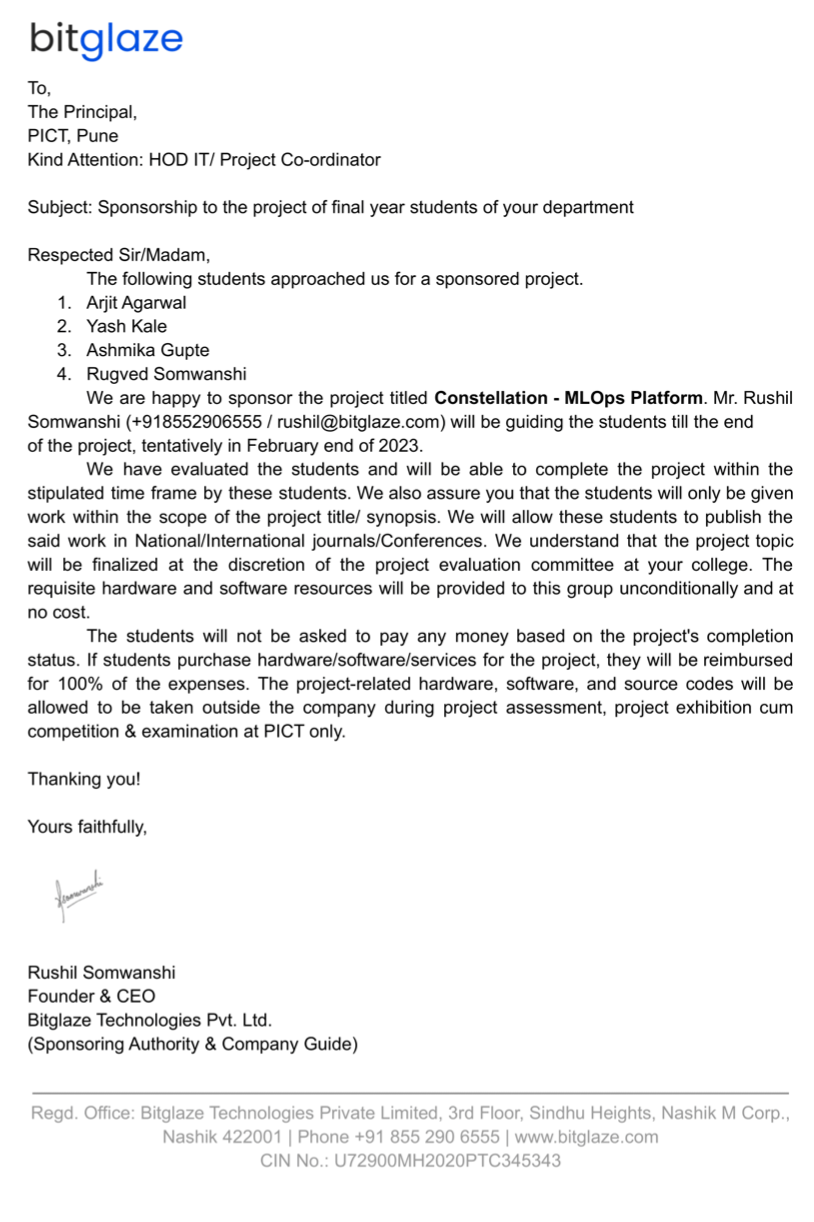
\includegraphics[]{Sponsorship_letter.png}
\addcontentsline{toc}{section}{Sponsorship letter}
%-----------------------------------Abstract------------------------------------------
		\newpage					%start a new page
		\pagestyle{plain}           %dont display header footer and display page nos
		\begin{center}				%centre align the text
			\begin{LARGE}
						\section*{ Abstract}
			%\vspace{.15 in}       %leave space of 0.5 inches vertically
			\end{LARGE}
		\end{center}
		\begin{normalsize}
{\setlength{\baselineskip}{1.1\baselineskip}   %set line spacing as 1.5
\noindent % Start writing abstract from here.
Constellation is a web-based MLOps platform, which aims to simplify and streamline the process of building and deploying machine learning pipelines for data scientists. The platform is designed to automate the preprocessing pipeline and use AutoML to identify the best model for a given dataset and task. The platform also provides a user-friendly interface for comparing and selecting the best-performing model. Constellation addresses the major challenge of deploying and monitoring ML pipelines by completely automating the process. The platform's ability to create highly accurate preprocessing pipelines and generate working Python code makes it a valuable tool for data scientists looking to optimize their workflow and achieve optimal results. Constellation has been identified to be used in various use cases like rapid prototyping and education.\\\\ 
\textbf{Keywords:} % start writing Keywords from here
MLOps, AutoML, Machine Learning, Low-Code\\\\
\par}
		\end{normalsize}
\addcontentsline{toc}{section}{Abstract}
%---------------------------------Abstract ends---------------------------------------
\newpage

\thispagestyle{empty}
\fancyhead{}
\renewcommand{\headrulewidth}{0pt}
%\fancypagestyle{plain}{}%start a new page
%		\thispagestyle{plain} 

\addcontentsline{toc}{section}{Contents}
\tableofcontents	 								% auto generate table of contents
\newpage
{\setlength{\baselineskip}{1.1\baselineskip}        % auto generate list of figures  
\listoffigures
\addcontentsline{toc}{section}{List of Figures}   % add to table of contents
}
\newpage
{\setlength{\baselineskip}{1.1\baselineskip}        % auto generate list of tables   
\listoftables
\addcontentsline{toc}{section}{List of Tables}
}
%---------------------------Abbrevations------------------------------------------------------------
\newpage
		\begin{LARGE}
			\begin{flushleft}
				\section*{\centering{Abbreviations}}
			\end{flushleft}
		\end{LARGE}
		\addcontentsline{toc}{section}{Abbreviations}	
\begin{normalsize}
					\noindent
{\setlength{\baselineskip}{1.1\baselineskip}
\vspace{0.2 in}
\begin{tabular}{lll}
\vspace{0.1 in}
MLOps	&	:	&	Machine Learning Operations	\\
\vspace{0.1 in}
ML	&	:	&	Machine Learning	\\
\vspace{0.1 in}
API	&	:	&	Application Programming Interface	\\
\vspace{0.1 in}
CV	&	:	&	Computer Vision\\
\vspace{0.1 in}
CVOps	&	:	&	Computer Vision Operations\\
\vspace{0.1 in}
SDK	&	:	&	Software Development Kit\\
\vspace{0.1 in}
GUI	&	:	&	Graphical User Interface\\
\vspace{0.1 in}
SD	&	:	&	Standard Deviation\\
\end{tabular}
\par}
\end{normalsize}

%-----------------------------------Chapter 1 Introduction}
\newpage
%\clearpage
\pagestyle{fancy}							%display header, footer
\pagenumbering{arabic}	%display page numbers in arabic
\renewcommand{\headrulewidth}{0.5pt}
\fancyhead[RO]{\textit{Constellation - an MLOps platform }} %set header to right
\fancyhead[LO]	{}											 %set header to left	
\renewcommand{\footrulewidth}{0.5pt}		% print horizontal line in the footer of 0.5 pt
\fancyfoot[RO]{\textit{Dept. of Information Technology}}		%set footer to right
\fancyfoot[LO]{\textit{PICT,Pune}}			%set footer to left
\fancypagestyle{plain}{}
\pagenumbering{arabic}	
\chapter{\centering{Introduction}}
\begin{normalsize}
			\noindent

%-------------------------------------------------------------------------------------------------------
%  Start writing from here.=
%(short para about your area describing its place in the world of Technology)
\section{Introduction} 	
{\setlength{\baselineskip}{1.1\baselineskip}
Constellation is a MLOps platform that centralizes your Machine Learning projects in one single place and helps accelerate ML development for small teams as well as large organizations. It makes creating and deployment of ML models easier and faster by minimising code and maximising intractability.
}	
\section{Motivation}
{\setlength{\baselineskip}{1.1\baselineskip}
%Start writing from here.
Machine learning has become a popular solution for solving real-world problems since the term was coined in 1959 \cite{b1}. Despite the similar workflow that an ML engineer follows on a daily basis, the process involves multiple critical steps such as data collection, preprocessing, feature selection, model identification, experimentation, hyperparameter tuning, result comparison, model selection, API development, cloud service implementation, analytics and monitoring, and continuous performance evaluation.
\par
Working with real-world data can be difficult due to its unclean nature, requiring substantial preprocessing before model training. Many preprocessing steps overlap regardless of the model, and comparing the performance of different models can be a challenging task. Hyperparameter tuning is a challenging process, and versioning on commonly used tools can be complicated when comparing different parameter configurations.
\par
It is critical to develop APIs for integrating a chosen model into an existing infrastructure, survey cloud service providers for deployment, set up analytics and monitoring, and continuously evaluate performance once a model is selected. These persistent issues are frequently encountered by both students and ML engineers in the industry \cite{b2}.
\par
As automation becomes more prevalent, there is an increasing need for a more efficient approach to avoid these repetitive and complex cycles. This project, 'Constellation,' aims to provide an MLOps platform that addresses these challenges and streamlines the machine learning workflow for both students and professionals in the industry.
\par}	

\section{Objectives}
{\setlength{\baselineskip}{1.1\baselineskip}
%Start writing from here.
Constellation is an MLOps Platform that consists of two main parts - an SDK and a Web Platform. The Platform and SDK work together to create an end-to-end data independent MLOps platform which will enable small to large-scale enterprises to create robust and scalable ML solutions with well-defined workflows. There are six main objectives of the project:
\begin{enumerate}
\item To enable quick visualization of the user's database.
\item To build a user-friendly graphical user interface for graphing and building machine learning pipelines, from data preprocessing to model selection and hyperparameter tuning.
\item To build an SDK which enables code generation of the given graphs built using the user interface.
\item To offer an auto-ML functionality to help novice users quickly get started with their tasks.
\item To help users easily compare and analyze different experiment and project metrics  easily in a collaborative space.
\item To enable deploying of the trained ML models on the cloud and monitoring their performance and usage.
\end{enumerate}
}
\section {Scope}
{\setlength{\baselineskip}{1.1\baselineskip}
%Start writing from here.
The project aims to develop an MLOps platform called 'Constellation' that consists of two main components - an SDK and a Web Platform. The primary goal of the project is to simplify the machine learning workflow and provide users with a comprehensive platform that caters to all their ML needs.
\par
The platform and SDK will work together to create an end-to-end data-independent MLOps platform that enables small to large-scale enterprises to build robust and scalable ML solutions with well-defined workflows. The platform will have a user-friendly graphical user interface for building machine learning pipelines, from data preprocessing to model selection and hyperparameter tuning. It will also offer an auto-ML functionality to help novice users quickly get started with their tasks.
\par
In addition, the platform will provide users with the ability to easily compare and analyze different experiment and project metrics in a collaborative space. Once a model is selected, the platform will enable deploying of the trained ML models on the cloud and monitoring their performance and usage.
\par
Overall, the platform aims to address persistent issues faced by both students and ML engineers in the industry, including challenges in working with real-life data, tedious model comparison, difficult hyperparameter tuning, and versioning issues on commonly used tools. By automating these repetitive and complicated cycles, Constellation will provide users with a more efficient approach to machine learning.
}


%-----------------------Literature Survey & Discussion (Literature Survey)----------------
\newpage 
\chapter{\centering{Literature Survey}}
{\setlength{\baselineskip}{1.1\baselineskip}
%Start writing from here.
The literature reviewed for the purpose of this project is mentioned below : 
\begin{enumerate}
\item Sustainable MLOps: Trends and Challenges (2020)
\newline Summary: MLOps and its supporting software are gaining popularity but pose sustainability risks as they become more integrated into daily software operations. This article highlights key challenges to address for sustainable AI software

\item Who Needs MLOps: What Data Scientists Seek to Accomplish and How Can MLOps Help? (2021)
\newline Summary: There are three types of organizations: those that focus on utilizing data, those that build models, and those that manage models. MLOps is only advantageous when there is a requirement for regular retraining and redeployment

\item A Data Quality-Driven View of MLOps (2021)
\newline Summary: The study showcases the manner in which diverse aspects of data quality disseminate across multiple stages of machine learning advancement, and how MLOps pipelines can be effectively devised

\item MLOps - Definitions, Tools, and Challenges (2022)
\newline Summary: The document describes the functioning and constituents of MLOps systems, presents useful tools, and suggests a strategy that combines AutoML, explainability, and sustainability to address current obstacles

\item Machine Learning Operations: A Survey on MLOps Tool Support (2022)
\newline Summary: Although MLOps has the potential to decrease human involvement in software development, there is a deficiency in a completely operational platform

\item MLOps: Overview of Current State and Future Directions (2023)
\newline Summary: The article explores the industrialization of machine learning projects, emphasizing the principles of MLOps, and the difficulties that arise when deploying an ML project. It presents a collection of tools to simplify the release of ML projects in production
\end{enumerate}

\section{Existing Methodologies}
The field of machine learning operations (MLOps) has witnessed a remarkable surge in recent years, with several platforms emerging to support various stages of the machine learning pipeline. This section provides an extensive overview of some of the most popular MLOps platforms that share similarities with 'Constellation'.
\subsection{DataRobot}
DataRobot MLOps platform makes deploying, monitoring, and managing machine learning models in production easy by providing a centralized location for all deployed models. It supports many different programming languages and development environments and offers advanced algorithms and prototypes for feature extraction and data processing\cite{b3}. Moreover, the platform can automatically choose the best features and methods for each model, which speeds up the development process.

\subsection{CometML}
Comet ML is a platform for experimentation that enables users to try and monitor Machine Learning projects from start to finish\cite{b4}. Comet ML works in tandem with the most common Machine Learning libraries, including sci-kit-learn, Pytorch, Tensorflow, Keras, and others. It supports a variety of languages, including Python, Javascript, Java, R, and REST APIs. Comet focuses on three fundamental development elements: experiment management, model management, and production monitoring. Comet's highly customizable ML development platform enables data scientists and engineers to manage and improve models in a single user interface across the entire ML lifecycle. Users of Comet ML can compare experiments, work with others, and create reports.

\subsection{Kubeflow}
It is an open-source ML platform that organizes ML system artifacts on top of the Kubernetes system and facilitates the creation, deployment, and monitoring of ML apps through automated pipelines\cite{b5}. It enables a few ML frameworks and monitoring plugins. A custom TensorFlow training job operator for building ML models, a TensorFlow Serving container for exporting learned TensorFlow models to Kubernetes, and services for building and managing interactive Jupyter notebooks are all included in Kubeflow.

\subsection{Picsell.ia}
Picsellia is a Computer Vision-focused end-to-end, extremely scalable MLOps Platform\cite{b6}. Data management, experiment tracking, model deployment, and model monitoring are some of their characteristics.

\section{Research Gap Analysis}

 In case of DataRobot, some users find the platform complicated and expensive, and it lacks data versioning and pipeline versioning features. Another potential issue is that users need to upload data to DataRobot's servers, which could be a concern for sensitive data.
\par
In CometML, there is no usage-based pricing plan, rendering it inaccessible to low-budget projects and small businesses. There is also the problem of limited scalability. 
\par
Kubeflow also lacks functionality for data and pipeline versioning. It also presently only supports TensorFlow. Kubeflow, because it is built on Kubernetes, necessitates extensive infrastructure that is difficult to set up. As a result, small and medium-sized businesses opt not to use it.
\par
But Picsellia is only a CVOps tool. It also does not allow customization for seasoned ML Engineers\cite{b7}. In any case, there is no choice to use structured or textual data. The foundation. There is no established modular strategy for accessing data and storing artifacts. Larger groups will be hesitant to store artifacts and data on their platform.
\par
After studying different MLOps tools and comparing their features, we have identified several obstacles to the widespread adoption of MLOps. These include high costs, complexity in usage, extensive infrastructure requirements, and limited scalability. Users are also hesitant to upload sensitive data to the cloud and prefer to store such information locally.
We have realized that there is currently no MLOps platform that can address all these issues simultaneously, i.e., store data on local servers, be affordable, scalable, easy to use, and without extensive infrastructure requirements. Thus, there is a need for an MLOps platform that has an intuitive user interface and extensive support for ML libraries. Our analysis of various MLOps platforms has led us to the conclusion that there is a new research area for developing a fully automated user interface-based MLOps platform that can be utilized by domain experts and developers.

}

%---------------------------Analysis & Discussion----------------
\newpage 
\chapter{\centering{Requirement Specification and Analysis}}
{\setlength{\baselineskip}{1.1\baselineskip}
%Start writing from here.
\section{Problem Definition}
To create an end-to-end data independent MLOps platform which will enable small to large scale enterprises create robust and scalable ML solutions with defined workflows
\section{Scope}
The 'Constellation' project aims to develop an MLOps platform that simplifies the machine learning workflow and provides users with a comprehensive platform that caters to all their ML needs. It consists of two main components - an SDK and a Web Platform that work together to create an end-to-end data-independent MLOps platform. The platform will have a user-friendly graphical interface, offer an auto-ML functionality and allow easy comparison and analysis of different metrics. The aim is to address persistent issues faced by both students and ML engineers and provide users with a more efficient approach to machine learning.
\section{Objectives}
Here are the six main objectives of the Constellation MLOps Platform:
\begin{enumerate}
\item To enable quick visualization of the user's database.
\item To build a user-friendly graphical user interface for graphing and building machine learning pipelines, from data preprocessing to model selection and hyperparameter tuning.
\item To build an SDK which enables code generation of the given graphs built using the user interface.
\item To offer an auto-ML functionality to help novice users quickly get started with their tasks.
\item To help users easily compare and analyze different experiment and project metrics easily in a collaborative space.
\item To enable deploying of the trained ML models on the cloud and monitoring their performance and usage.
\end{enumerate}
\section{Proposed Methodology}
Constellation overcomes the shortcomings of other MLOps platforms by utilizing a unique methodology. First, it provides a user-friendly graphical user interface (GUI) that enables users to create machine learning pipelines easily. The GUI allows users to design, build, and visualize their pipelines from data preprocessing to model selection and hyperparameter tuning.
\par
Second, Constellation includes an SDK that generates code from the user's pipeline, enabling users to reuse their code and replicate their experiments easily. The SDK also provides an auto-ML functionality that helps novice users to quickly get started with their tasks.
\par
Third, Constellation provides a collaborative space for users to compare and analyze different experiment and project metrics easily. It includes extensive support for ML libraries, and users can visualize their results with various charts and graphs.
\par
Finally, Constellation enables the deployment of trained ML models on the cloud and monitoring their performance and usage. This methodology ensures that users can create robust and scalable ML solutions with well-defined workflows, addressing the persistent issues faced by both students and ML engineers in the industry.
\section{Project Requirements}
\subsection{Datasets}
The platform currently supports '.csv' files only. The user can upload their dataset in the 'Data Lake' section.
\subsection{Functional Requirements}
The functional requirements of Constellation are :
\begin{enumerate}
\item Data Visualizer
\item  UserInterface for graphing and building machine learning pipelines
\item AutoML functionality
\item User Interface easily compare and analyze different experiment and project metrics.
\item Model Deployment and Monitoring
\end{enumerate}
\subsection{Non Functional Requirements}
The non-functional requirements of Constellation are :
\begin{enumerate}
\item Security
\item Accuracy
\item Collaboration
\item Usability
\end{enumerate}
\subsection{Hardware Requirements}
The hardware requirements of Constellation are :
\newline
\textbf{Amazon EC2 T2 instances}
\newline Features included in this instance is as follows:
\begin{itemize}
    \item Up to 3.3 GHz Intel Xeon Scalable processor (Haswell E5-2676 v3 or Broadwell E5-2686 v4)
    \item High frequency Intel Xeon processors
    \item Burstable CPU, governed by CPU Credits, and consistent baseline performance
    \item Balance of compute, memory, and network resources
\end{itemize}
\subsection{Software Requirements}
The software requirements of Constellation are :
\begin{enumerate}
\item \textbf{Python}\\
The 'humble' SDK is being used for the platform, which is written in Python.
\item \textbf{Pandas}\\
Pandas is used as a data reading and preprocessing tool for structured data.
\item \textbf{Scikit Learn}\\
We are using the scikit learn library to implement various machine learning models for the SDK.
\item \textbf{Next.js}\\
Next.js is an open-source Frontend web development framework which makes the prototyping of our platform extremely quick and with minimal impact to performance.
\item \textbf{Nest.js}\\
Nest.JS is a framework that helps build Node.JS server-side applications. It is a highly scalable and fast backend framework.
\item \textbf{PostgreSQL}\\
PostgreSQL is an extremely well-known and widely used relational database system. It provides a rich feature set.
\item \textbf{Docker}\\
Docker enables us to provide a template structure to run for the target system. It guarantees that the target system will run the intended code properly.
\item \textbf{AWS}\\
Amazon Web Services (AWS) is a web server hosting platform. We intend to use it to make training accessible to individuals who do not want to run/deploy their ML model on their own system.
\end{enumerate}
\section{Project Plan}
\subsection{Project Resources}
\subsection{Module Split-up}
The different modules of Constellation are :
\begin{enumerate}
\item \textbf{Huble} : The SDK that works with Constellation's Web Platform top convert graphical pipelines to Python Code
\item \textbf{Activity Page} : Gives a quick overview of the activities and workspaces of the user and other collaborators.
\item \textbf{Data Lake} : The users can upload their datasets in this section. It contains a list of datasets. This page contains : 
\begin{enumerate}
\item Dataset visualizer 
\item Dataset description and analytics
\end{enumerate}
\item \textbf{Workspaces} : Allows users to organize their projects. Each workspace can contain multiple projects. Each project is associated with a task and primary dataset. Each project contains :
\begin{enumerate}
\item A list of experiments
\item AutoML
\item Compare Experiments Page
\item Builder to create new experiment pipelines
\end{enumerate}
\item \textbf{Model Registry} : Contains a list of models supported by Huble SDK, and their short description.
\item \textbf{Deployments Page} : Contains a list of deployed models with quick overview of their health. Each deployment page contains :
\begin{enumerate}
\item Monitoring Analytics
\item Docker logs
\item Try it Out Interface
\end{enumerate}
\item \textbf{Profile Page} : Gives an overview of the user specific metrics.
\end{enumerate}
\subsection{Functional Decomposition}
\begin{figure}[H]
    \centering
    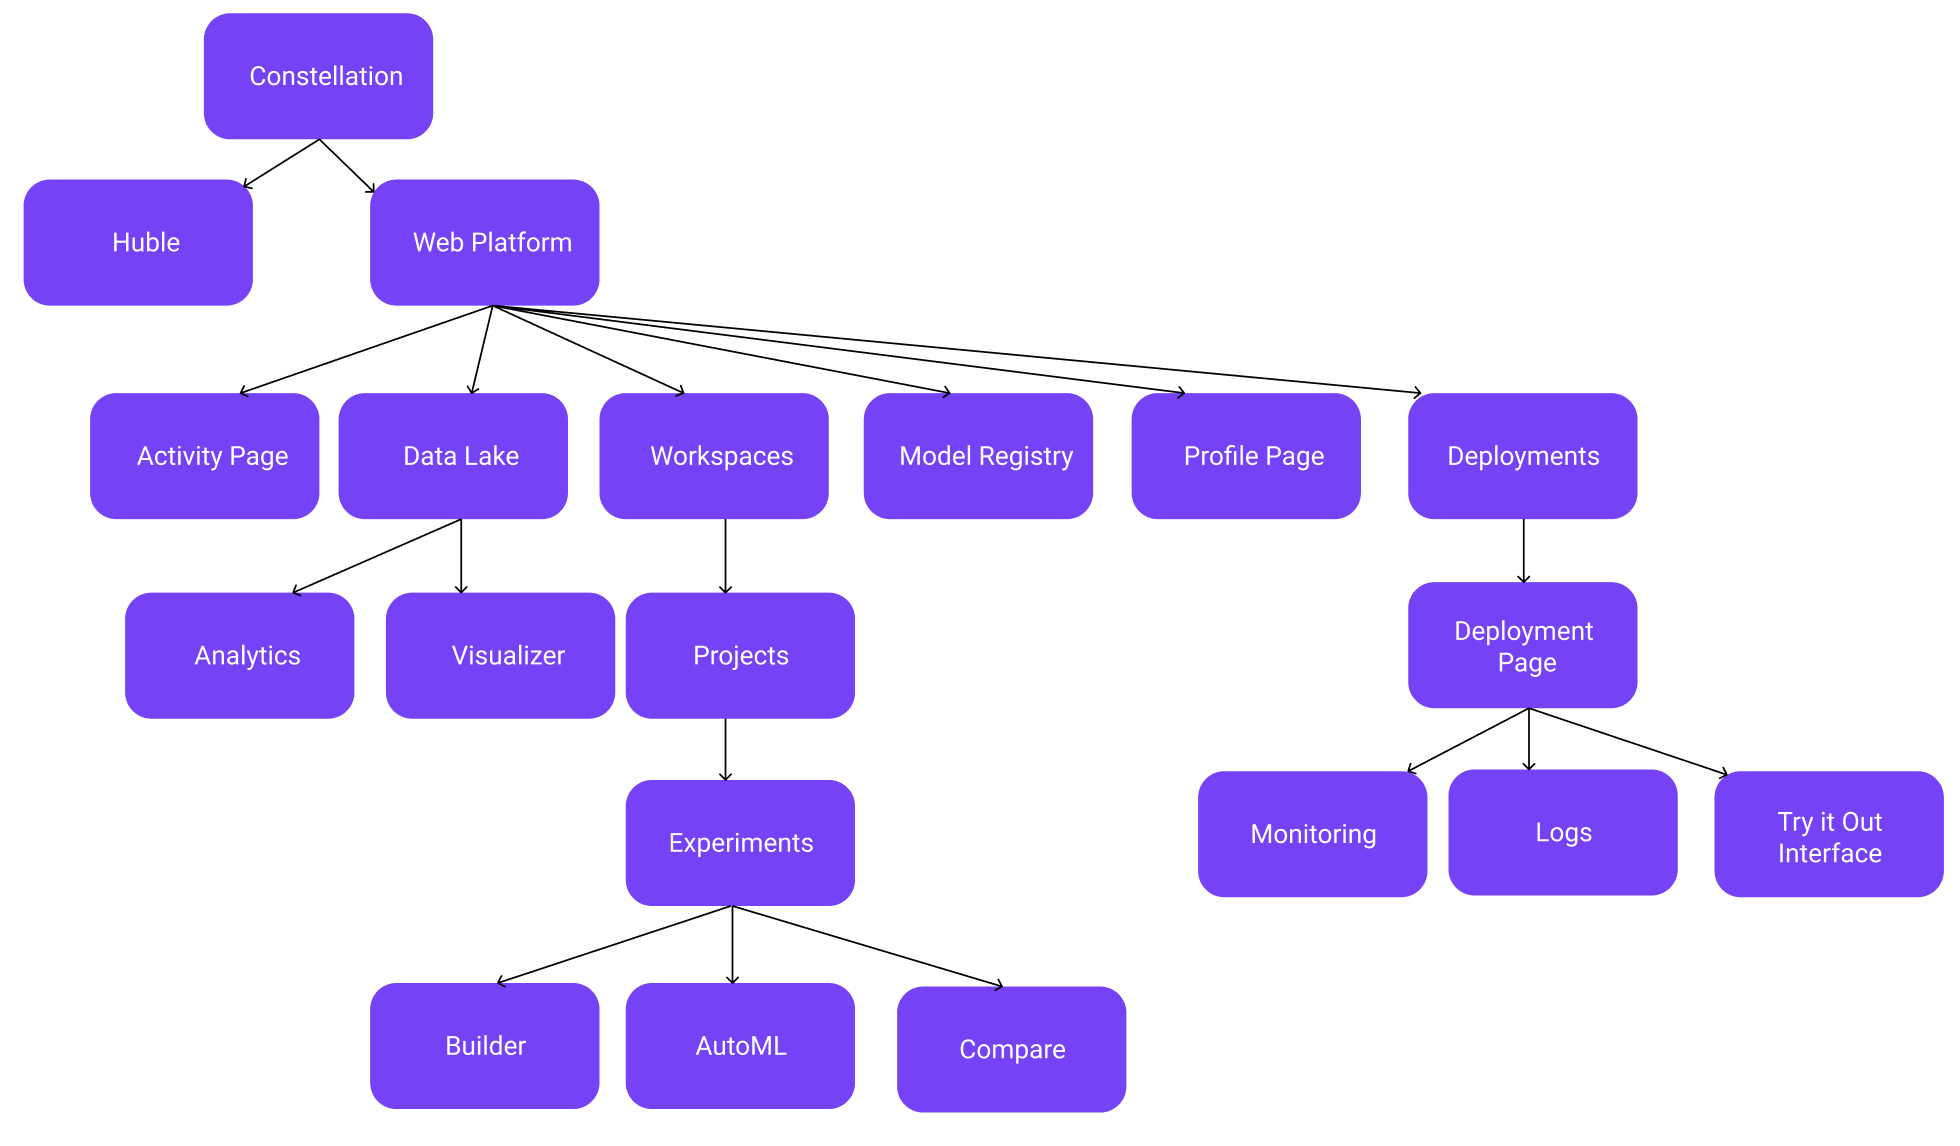
\includegraphics[scale=0.5]{diagrams/Functional_decomposition.png}
        \caption{Functional decomposition of Constellation Modules}
    \label{}
\end{figure}
\subsection{Project Team Role and Responsibilities}
Team Roles were assigned as follows :
\begin{table}[h]
\centering
\begin{tabular}{|c|c|c|}
\hline
\textbf{Team Member} & \textbf{Role} & \textbf{Responsibilities} \\ \hline
Arjit Agarwal & 
Full Stack Developer &
\begin{tabular}[c]{@{}c@{}}
Compare Page\\ 
Experiment Builder\\ 
AutoML UI
\end{tabular} \\ \hline
Ashmika Gupte & 
Python Developer &
\begin{tabular}[c]{@{}c@{}}
AutoML\\ 
Huble SDK
\end{tabular} \\ \hline
Rugved Somwanshi &  
Full Stack Developer &
\begin{tabular}[c]{@{}c@{}}
Utils\\ 
Data Lake\\ 
Deployments Page\\ 
Experiment Builder\\ 
SDK Integration
\end{tabular} \\ \hline
Yash Kale & 
Full Stack Developer &
\begin{tabular}[c]{@{}c@{}}
Utils\\ 
Dataset Visualizer\\ 
Deployments Page\\ 
Experiment Builder
\end{tabular} \\ \hline
\end{tabular}
\caption{Team Roles and Responsibilities}
\end{table}

\subsection{Project Plan 3.0}
\subsection{PERT Table}

\begin{table}[htbp]
    \centering
    \caption{PERT Table for Project Tasks}
    \label{tab:pert-table}
    \begin{tabular}{|l|c|c|c|c|c|}
        \hline
        \textbf{Task} & \textbf{Predecessor} & \textbf{Optimistic} & \textbf{Estimated} & \textbf{Pessimistic} \\
        \hline
        Research Existing Platforms(A) & - & 4 & 5 & 6  \\
        \hline
        Literature Survey(B) & A & 1 & 2 & 3  \\
        \hline
        Basic Website Setup(C) & B & 0.5 & 1 & 1.5  \\
        \hline
        Finalize UI Components(D) & C & 1.5 & 2 & 2.5  \\
        \hline
         Create Basic Backend(E) & C & 1.5 & 2 & 2.5  \\
        \hline
        Create Pipeline Builder(F) & D,E & 1 & 2 & 3 \\
        \hline
        Create Projects and Experiments(G) & F & 1 & 2 & 3  \\
        \hline
        Train Model Functionality(H) & G,I & 0.5 & 1 & 1.5 \\
        \hline
        Create Huble SDK(I) & B & 4 & 6 & 8  \\
        \hline
        Compare Experiments Page(J) & H & 1 & 2 & 3  \\
        \hline
        AutoML Implementation(K)& K & 3 & 4 & 5 \\
        \hline
    \end{tabular}
\end{table}


\subsection{PERT Diagram}

\begin{figure}[H]
    \centering
    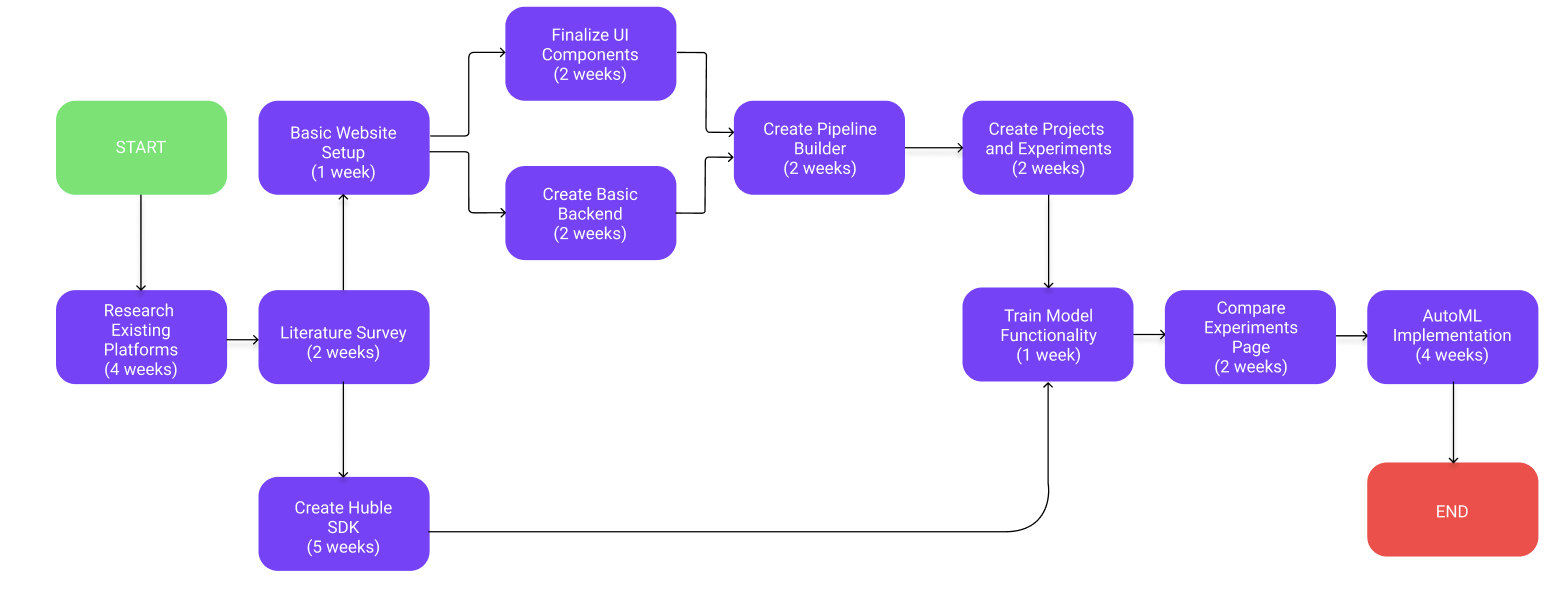
\includegraphics[scale=0.65]{diagrams/PERT.png}
        \caption{PERT Diagram}
    \label{}
\end{figure}
%Start writing from here.

%---------------------------Proposed solution & its Design--------------
\newpage 
\chapter{\centering{System Analysis and Design}}
{\setlength{\baselineskip}{1.1\baselineskip}

%---------- Proposed Solution
%those who have done implementation can 
\section{System Architecture}
{\setlength{\baselineskip}{1.1\baselineskip}
%Start writing from here.

\begin{figure}[H]
    \centering
    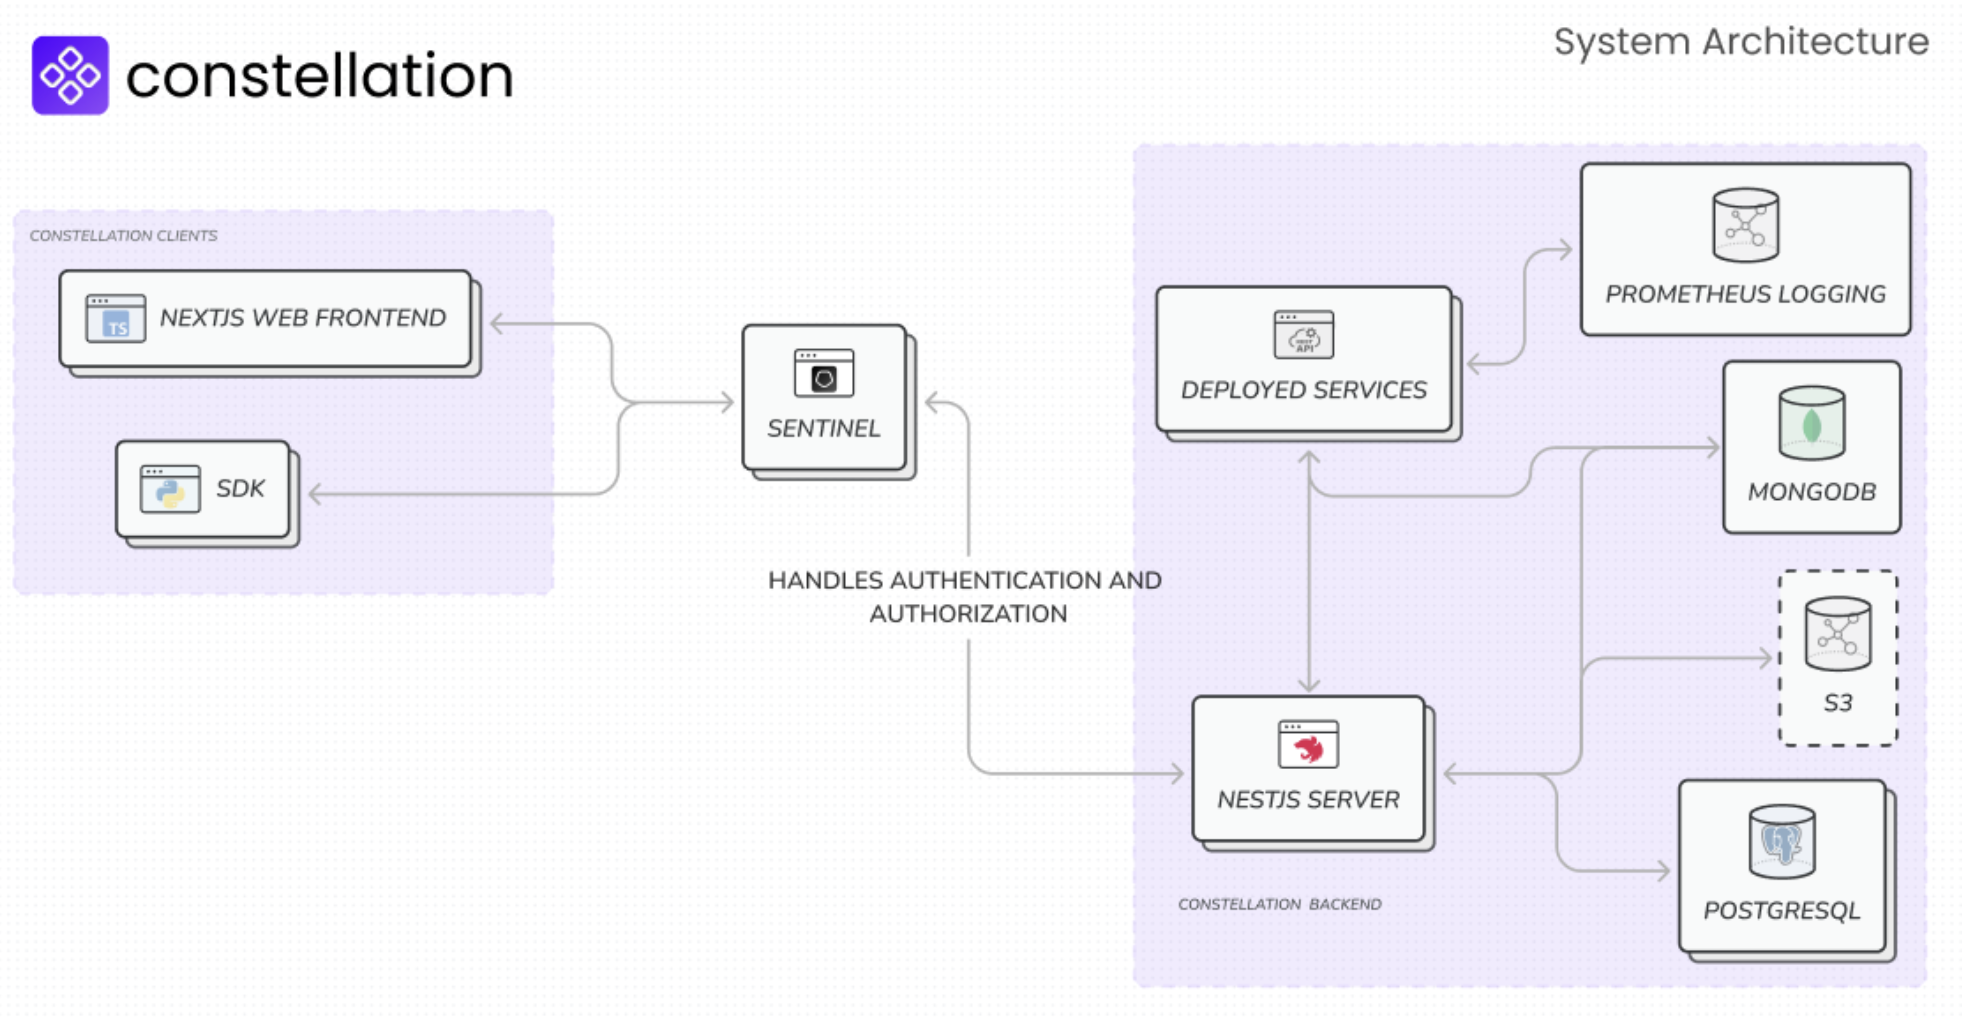
\includegraphics[scale=0.5]{diagrams/System_architecture.png}
        \caption{System Architecture}
    \label{}
\end{figure}
}
\section{Necessary UML Diagrams}
{\setlength{\baselineskip}{1.1\baselineskip}
%Start writing from here.
\subsection{Use Case Diagram}
\begin{figure}[H]
    \centering
    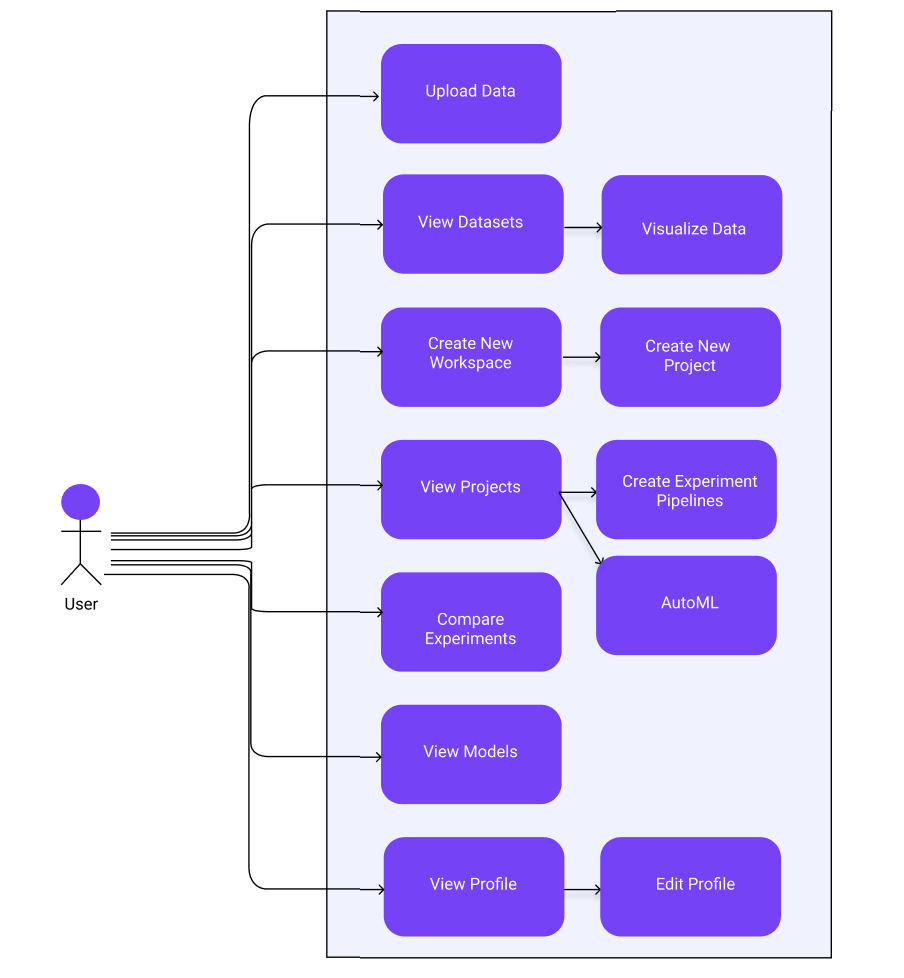
\includegraphics[scale=0.9]{diagrams/Use_case_diagram.png}
        \caption{Use Case Diagram}
    \label{}
\end{figure}
\subsection{DFD}
\subsection{Activity Diagram}
\begin{figure}[H]
    \centering
    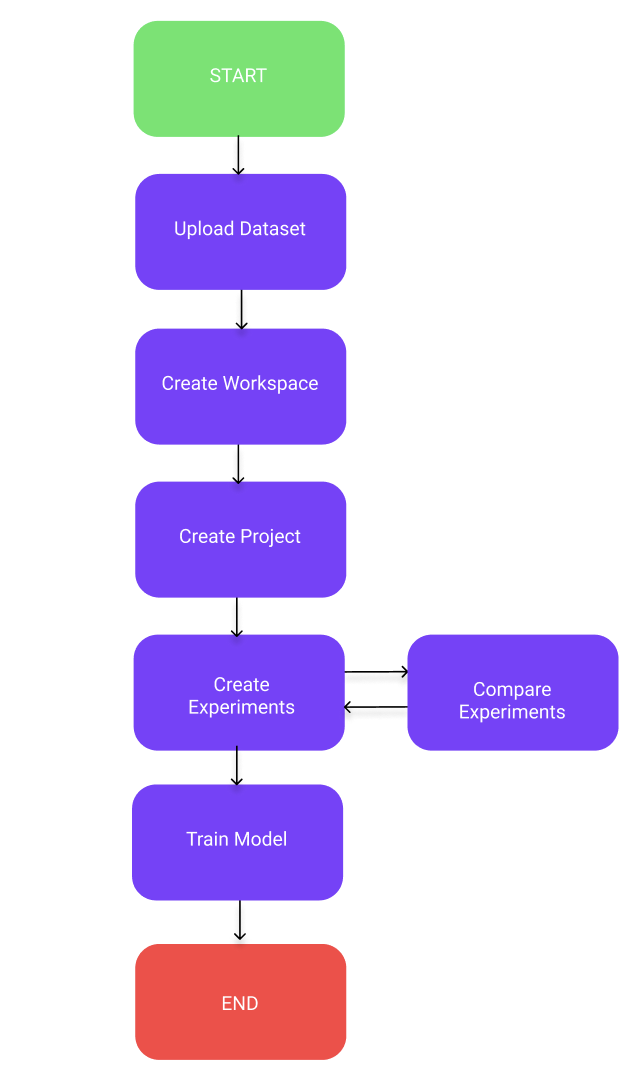
\includegraphics[scale=0.9]{diagrams/Activity_diagram.png}
        \caption{Activity Diagram}
    \label{}
\end{figure}
\subsection{Sequence Diagram}
\begin{figure}[H]
    \centering
    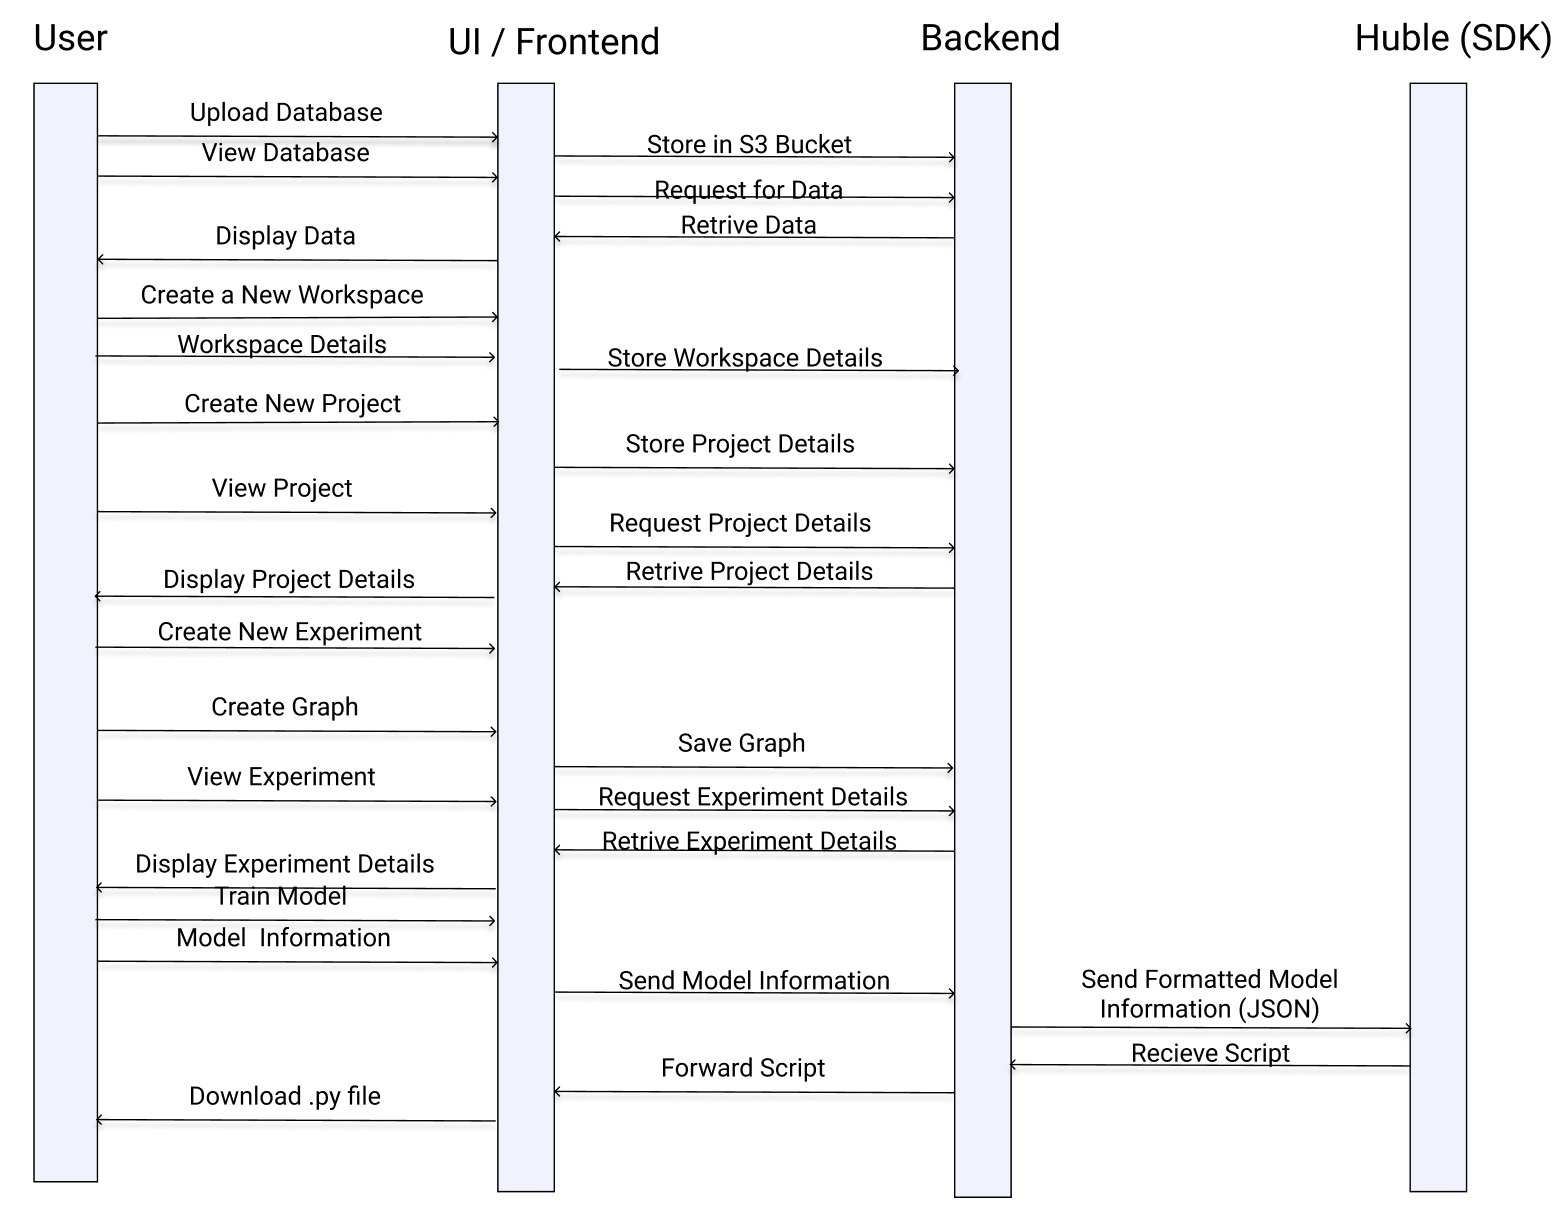
\includegraphics[scale=0.6]{diagrams/Sequence_diagram.png}
        \caption{Sequence Diagram}
    \label{}
\end{figure}

\section{Algorithm and Methodologies}

}


%---------------------------Implementation ----------------
\newpage 
\chapter{\centering{Implementation}}
{\setlength{\baselineskip}{1.1\baselineskip}
%Start writing from here.
\section{Stages of Implementation}

\subsection{Dataset collection and Analysis}
Every ML project begins with a dataset that can be difficult to gather and manage. Furthermore, the same dataset can be used by multiple users in their own workspaces. Constellation provides a seamless process that is designed to help users accumulate data, manage their datasets, and perform feature analysis by plotting various charts. The platform accepts data uploaded in CSV format and is saved in a cloud-based store (AWS
S3 bucket). A GUI explains various metrics pertaining to the dataset like column data types, date of dataset creation, etc. Users can examine raw data in each dataset through time series plots, bar charts, line charts, etc according to the data types.
\begin{figure}[H]
    \centering
    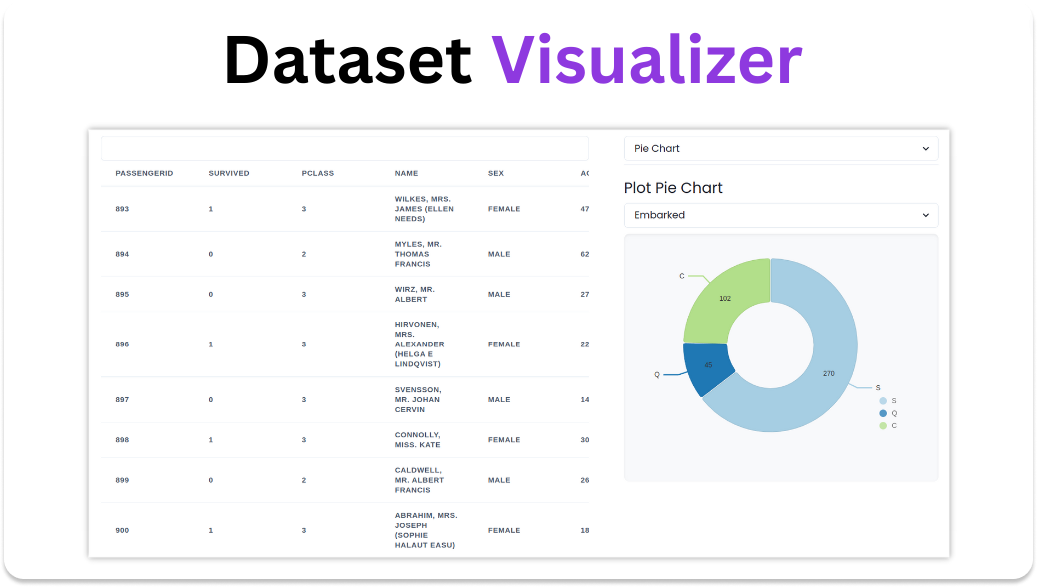
\includegraphics[scale=0.4]{diagrams/Visualizer.png}
    \caption{Visualizer}
    \label{}
\end{figure}
\subsection{Drag N Drop Training Pipeline}
One of the major features provided by Constellation that sets it apart from other MLOps platforms is the "Drag N Drop" feature included in the training pipeline. The entire ML training pipeline can be divided into individual processes called data preprocessing, training, and evaluation. These processes can be further divided into individual lines of code which run on the dataset. The fundamental blocks called "nodes" implement different features like models and essential nodes. The figure below represents it properly.
\begin{figure}[H]
    \centering
    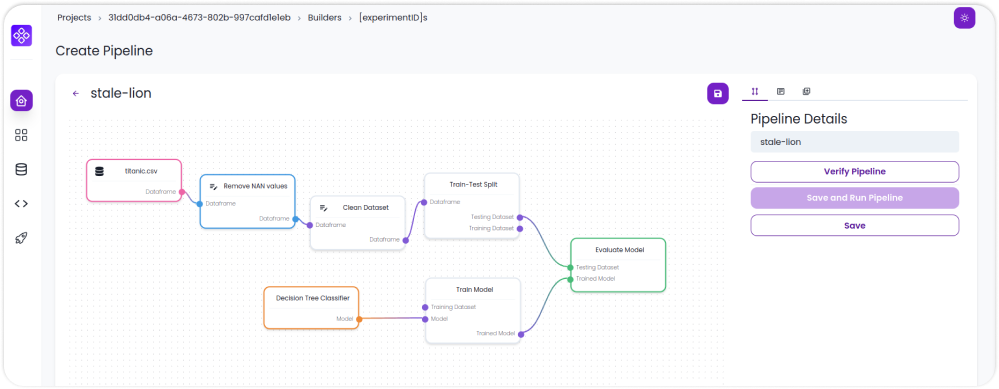
\includegraphics[scale=0.4]{diagrams/Builder.png}
    \caption{Graph UI}
    \label{}
\end{figure}
\subsection{Code Generation}
The ML pipelines made on the graph need to be converted into code. For this, the Huble SDK is used. The SDK parses the graph JSON and converts it into code by templating. A direct acyclic graph code generation algorithm has been implemented for the same. The code snippet is shown below. 
\newline

\lstset{
  language=Python,
  basicstyle=\ttfamily,
  keywordstyle=\color{blue},
  commentstyle=\color{green!40!black},
  stringstyle=\color{purple},
  showstringspaces=false,
  breaklines=true,
  frame=single,
  captionpos=b,
  numbers=left,
  numberstyle=\tiny\color{gray},
  escapeinside={(*@}{@*)}
}

\begin{lstlisting}
g = Graph(len(graph["nodes"]))
graph_dict = {}
for i in graph["nodes"]:
    graph_dict[(i["data"]["name"])] = i
map = {}
j = 0
while j < (len(graph["nodes"])):
    for i in graph["nodes"]:
        map[(i["id"])] = j
        j += 1
map2 = {y: x for x, y in map.items()}
for i in graph["edges"]:
    g.addEdge(map[i["source"]], map[i["target"]])
res = g.topologicalSort()
steps = []
for i in res:
    steps.append(map2[i])
steps_list = {}
for i in steps:
    for j in range(len(graph["nodes"])):
        if i == graph["nodes"][j]["id"]:
            steps_list[(graph["nodes"][j])] = 
            graph["nodes"][j]["node_type"]
if colab:
    output_file = "/content/output.py"
else:
    output_file = "output.py"
return generate_code(steps_list)
\end{lstlisting}


\subsection{Deployments}
Docker-in-docker is used to create docker containers inside the same network and use file-sync volumes to make sure Prometheus detects all new servers created to monitor. This provides extensive flexibility for us to implement cloud-agnostic features in the future. 
\begin{figure}[H]
    \centering
    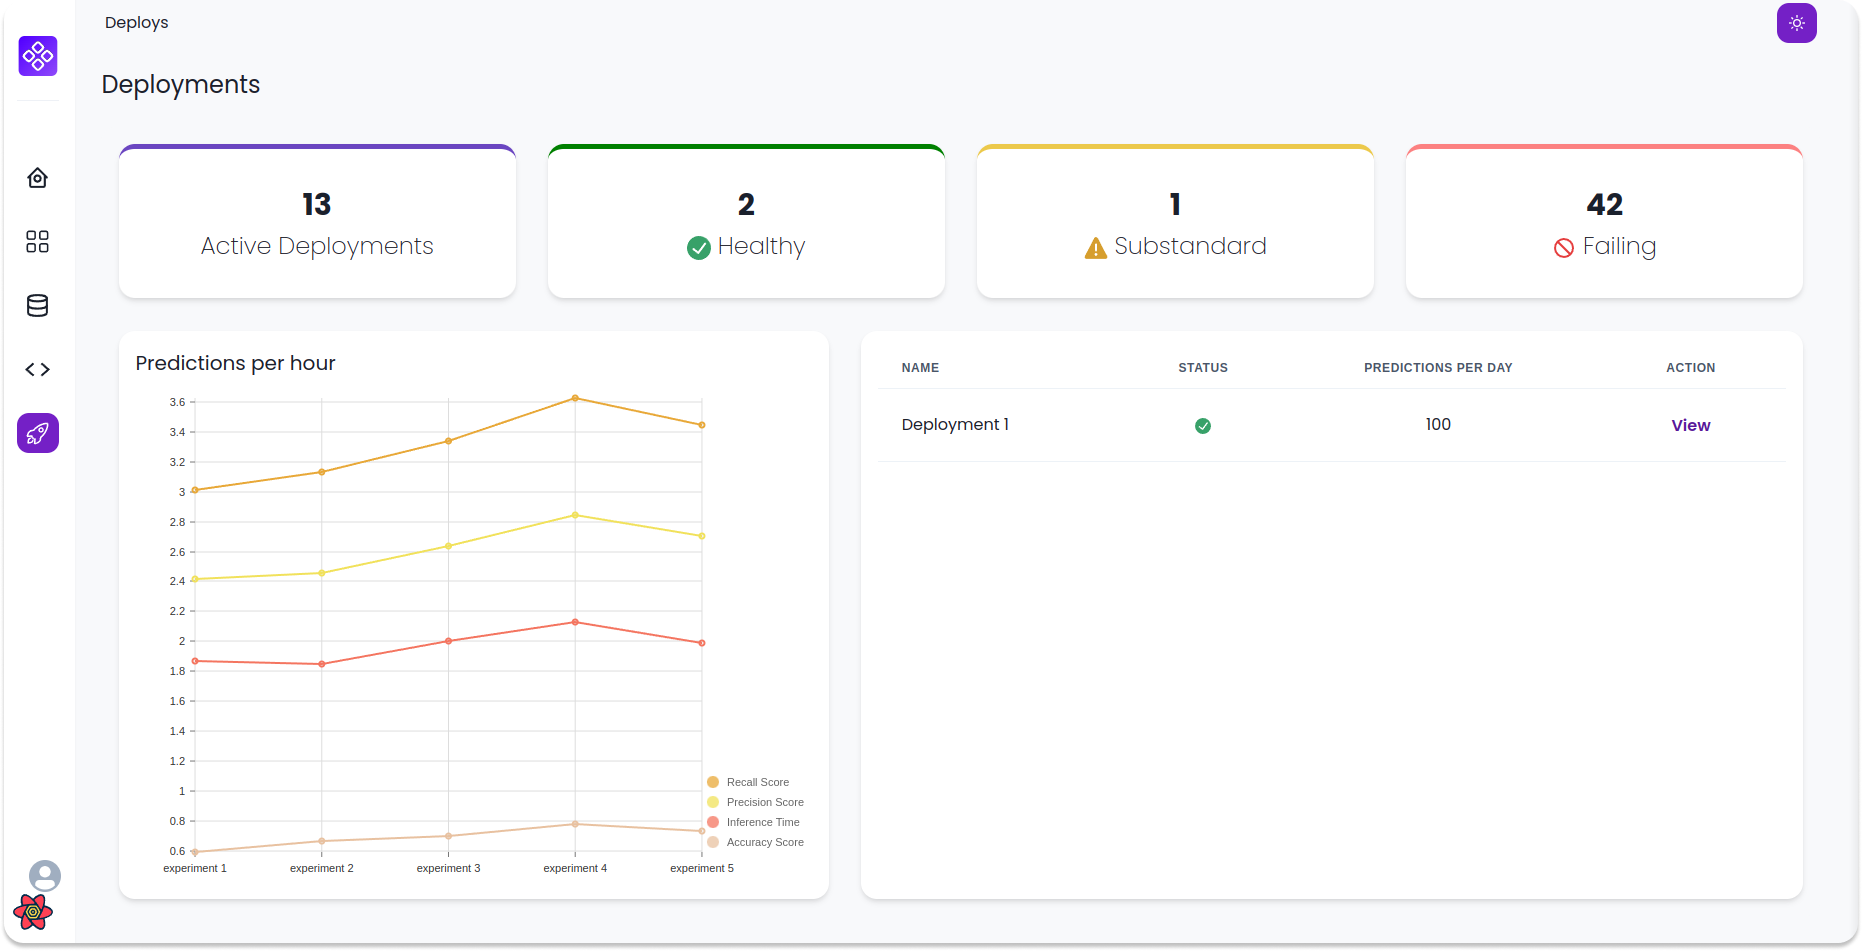
\includegraphics[scale=0.2]{diagrams/Deployments.png}
    \caption{Deployments}
    \label{fig:builder}
\end{figure}
\begin{figure}[H]
    \centering
    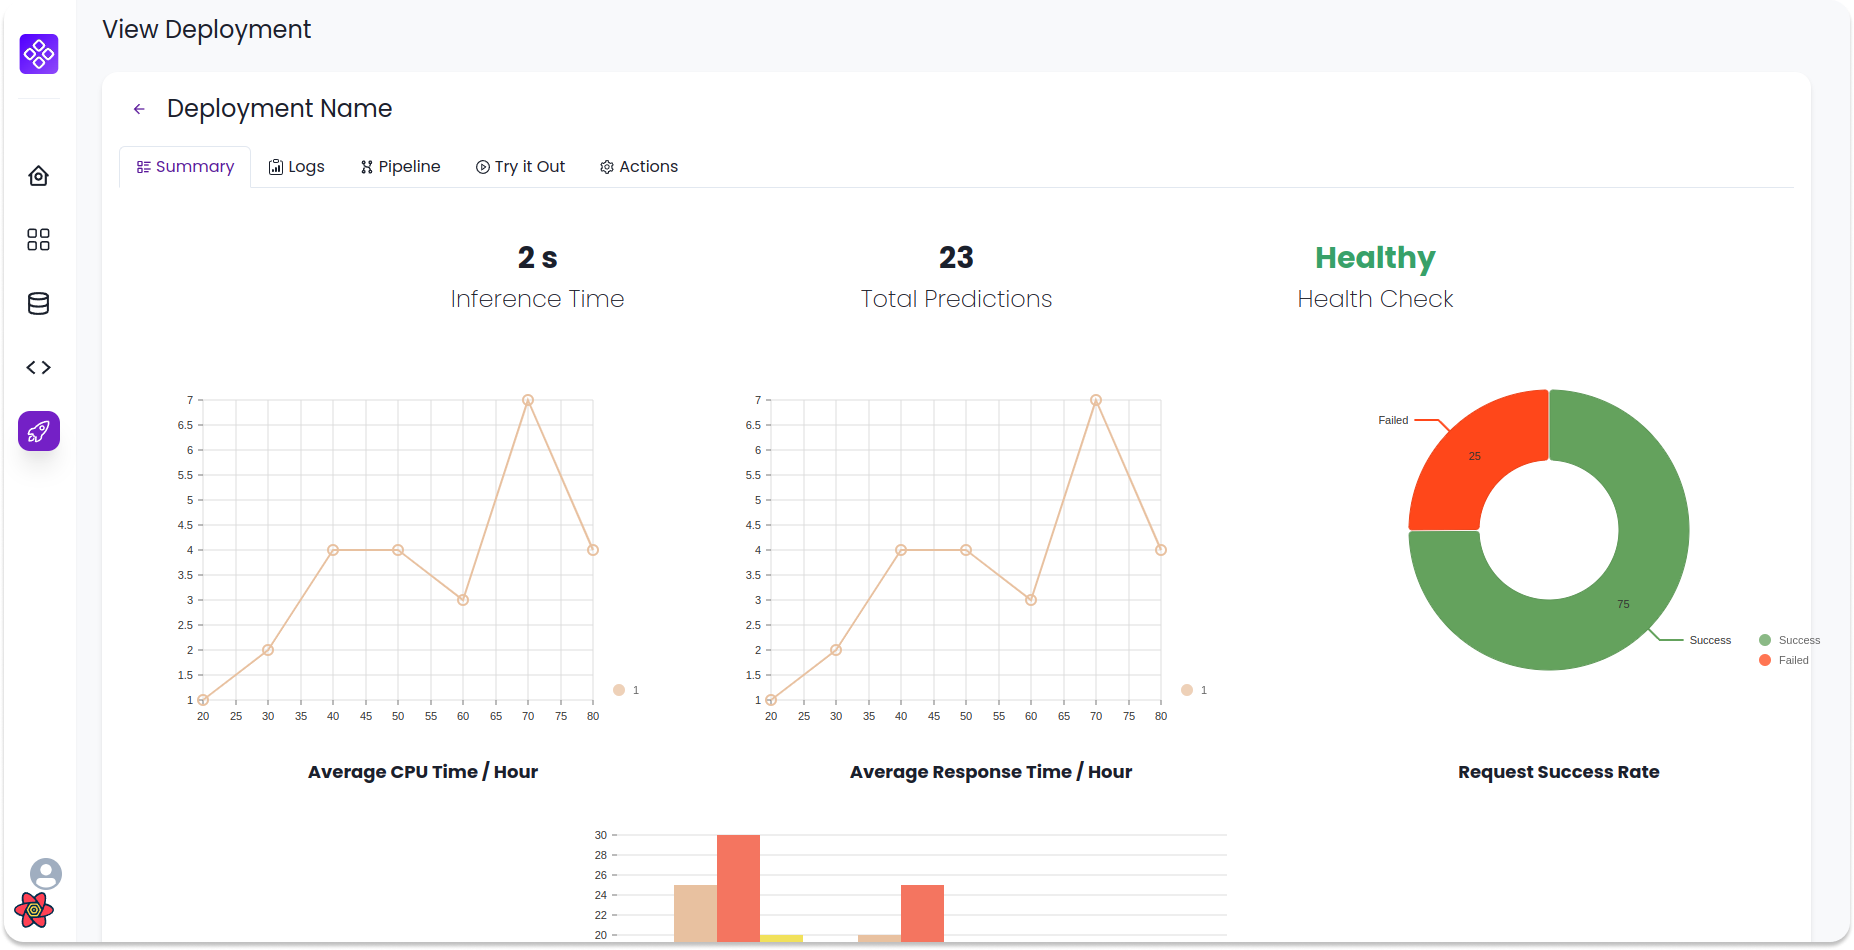
\includegraphics[scale=0.2]{diagrams/View_deployments.png}
    \caption{View Deployments }
    \label{fig:builder}
\end{figure}
\par


%------------Results-------------------- 
\newpage 
\chapter{\centering{Results}}
{\setlength{\baselineskip}{1.1\baselineskip}
%Start writing from here.
\section{Results of Experiments }
\section{Result Analysis }
After conducting unit, integration, white box, and black box testing on the Constellation web application, we are pleased to report that the system is working as expected.

In unit testing, all individual components were tested to ensure that they are functioning properly. The tests showed that each component is functioning as expected without any issues.

Integration testing was performed to verify that the different components of the system are working together seamlessly. The tests showed that the components are integrated well and are communicating with each other as expected.

White box testing was conducted to ensure that the internal logic of the system is working as intended. The tests showed that the code is properly structured and the internal logic is functioning correctly.

Finally, black box testing was conducted to verify that the system is meeting its functional requirements. All test cases passed successfully, indicating that the system is meeting all its functional requirements.

Overall, the results of the testing indicate that the Constellation web application is working as expected and meets the required specifications. We recommend that the system can now be deployed to production.
\section{Testing}
\subsubsection{White Box}
\begin{table}[h]
\centering
\caption{White Box Testing Results for Constellation}
\label{tab:whitebox}
\begin{tabular}{|c|c|c|c|}
\hline
 \textbf{Test Case} & \textbf{Expected Result} & \textbf{Actual Result} \\ \hline
 Check input for experiment names & Error message  & Error message  \\ \hline
Check model training  & Trained model saved & Trained model saved \\ \hline
 Check database connection & Connection established & Connection established \\ \hline
 Check  Builder functionality & Pipeline built successfully & Pipeline built successfully \\ \hline
 Check AutoML functionality & Optimal model  & Optimal model  \\ \hline
\end{tabular}
\end{table}

\subsubsection{Unit Testing}

\begin{table}[h!]
\centering
\caption{Unit Test Results for Constellation}
\label{tab:unit-test-results}
\begin{tabular}{|c|c|c|c|}
\hline
\textbf{Test Case ID} & \textbf{Test Description} & \textbf{Expected Result} & \textbf{Actual Result} \\ \hline
UT-01 & Loading of data & Data is loaded successfully & Pass \\ \hline
UT-02 & Preprocessing of data & Data is preprocessed correctly & Pass \\ \hline
UT-03 & Model training & Model is trained successfully & Pass \\ \hline
UT-04 & Model evaluation & Metrics are computed correctly & Pass \\ \hline
UT-05 & Deployment of model & Model is deployed successfully & Pass \\ \hline
\end{tabular}
\end{table}

\subsubsection{Integration Testing}
\begin{table}[H]
\centering
\caption{Integration Testing Results for Constellation}
\label{tab:integration-testing}
\begin{tabular}{|c|c|c|}
\hline
\textbf{Component} & \textbf{Test Cases Passed} & \textbf{Test Cases Failed} \\ \hline
Frontend & 20 & 0 \\ \hline
Backend & 18 & 1 \\ \hline
Database & 12 & 0 \\ \hline
SDK & 16 & 3 \\ \hline

\end{tabular}
\end{table}

\subsubsection{Black Box}
\begin{table}[h]
\centering
\caption{Black Box Testing Results for Constellation}
\label{tab:blackbox-results}
\begin{tabular}{|c|c|c|}
\hline
\textbf{Test Case} & \textbf{Input} & \textbf{Expected Output} \\ \hline
1 & Login credentials & Successful login \\ \hline
2 & Invalid login credentials & Error message displayed \\ \hline
3 & Dataset upload & Dataset successfully uploaded \\ \hline
4 & Invalid dataset format & Error message displayed \\ \hline
5 & Model training & Successful training \\ \hline
6 & Invalid hyperparameters & Error message displayed \\ \hline
7 & Prediction on test data & Successful prediction \\ \hline
8 & Invalid test data format & Error message displayed \\ \hline
\end{tabular}
\end{table}

\subsubsection{Test Cases}
\begin{enumerate}
\item\textbf{Test Case 1}
\begin{enumerate}
    \item \textbf{Description:} Verify that the user can successfully log in to the Constellation web application.
    \item \textbf{Preconditions:} The user is on the login page of the Constellation web application.
    \item \textbf{Inputs:} The user enters valid login credentials and clicks the "Login" button.
    \item \textbf{Actions:} The system logs the user in and displays the home page.
    \item \textbf{Expected Results:} The home page is displayed with the user's information and options to navigate to different pages within the application.
\end{enumerate}
\item\textbf{Test Case 2}
\begin{enumerate}
\item \textbf{Description:} Verify that the user can upload a dataset to the Constellation web application.
\item \textbf{Preconditions:} The user is logged in to the Constellation web application.
\item \textbf{Inputs:} The user navigates to the "Datasets" page and clicks the "Upload Dataset" button. The user selects a valid dataset file and clicks the "Upload" button.
\item \textbf{Actions:} The system uploads the dataset and displays a success message.
\item \textbf{Expected Results:} The uploaded dataset is displayed on the "Datasets" page with the correct information and options to view, edit, or delete the dataset.
\end{enumerate}

\item\textbf{Test Case 3}
\begin{enumerate}
\item \textbf{Description:} Verify that the user can create and run an experiment on the Constellation web application.
\item \textbf{Preconditions:} The user is logged in to the Constellation web application and has at least one dataset uploaded.
\item \textbf{Inputs:} The user navigates to the "Experiments" page and clicks the "New Experiment" button. The user selects a dataset and sets the experiment parameters. The user clicks the "Run Experiment" button.
\item \textbf{Actions:} The system creates the experiment, runs it, and displays the results.
\item \textbf{Expected Results:} The experiment is created and run successfully, and the results are displayed on the "Experiments" page with the correct information and options to view, edit, or delete the experiment.
\end{enumerate}
\item\textbf{Test Case 4}
\begin{enumerate}
    \item \textbf{Description:} Verify that the user can create a new project in the Constellation web application.
    \item \textbf{Preconditions:} The user is logged in to the Constellation web application and is on the home page.
    \item \textbf{Inputs:} The user clicks on the "New Project" button and enters the required information.
    \item \textbf{Actions:} The system creates a new project and displays it on the home page.
    \item \textbf{Expected Results:} The new project is displayed on the home page with the correct information entered by the user.
\end{enumerate}
\end{enumerate}
\subsubsection{Summary of Black Box Testing}
The table lists the test cases along with the input and the expected output for each test case. The test cases cover various functionalities of the application such as login, dataset upload, model training, and prediction. The expected outputs were compared to the actual outputs obtained during the testing phase. The black box testing helped to ensure that the application meets the requirements and functions as expected.

%----------Conclusion-----------------
\newpage 
\chapter{\centering{Conclusion and Future Scope}}
{\setlength{\baselineskip}{1.1\baselineskip}
%Start writing from here.
\section{Conclusion}

Constellation's advantages over traditional methods of machine learning model development and deployment make it a promising solution for organizations looking to adopt MLOps practices. The platform's user-friendly interface, automation of various stages of the machine learning pipeline, and detailed reporting and visualization capabilities offer a streamlined and efficient approach to machine learning development.
\par
Furthermore, Constellation's modular and scalable architecture makes it a versatile platform that can be customized to meet the unique needs of different organizations and applications. As the platform continues to evolve and address its limitations, it has the potential to become a valuable asset for data scientists and ML engineers worldwide.

\section{Limitations of the Project}
Constellation provides a user-friendly interface for data scientists to easily build, test, and deploy machine learning models. However, as with any complex technology, Constellation does face several challenges and limitations that need to be addressed. One of the primary limitations of Constellation is that it does not support distributed training of models, which can be a significant hindrance when dealing with large datasets or complex models. Additionally, Constellation does not currently support GPU processing, as the platform relies on the CPU-based Scikit-learn library.
\par
Another limitation of Constellation is that it only supports structured data, which can be a significant challenge when working with unstructured or multimedia data types. Furthermore, Constellation only supports one dataset in each pipeline, which can be limiting when working with more complex data analysis scenarios. While training for big data is possible, visualization of the data can be challenging, and there is a need for better integration with MLOps libraries.
\par
Moreover, a significant challenge for Constellation is to make it inclusive, where the existing workflows of ML engineers should not be disturbed. Another limitation of Constellation is that Arm processors cannot handle all models, as not all libraries are supported. While the experimental results demonstrate the effectiveness of Constellation, these challenges and limitations must be addressed to ensure the platform's continued success. Despite these limitations, Constellation represents a significant step forward in the field of MLOps and offers an intuitive and user-friendly platform for machine learning model development and deployment.
\section{Future Scope}
Constellation's current functionality is limited to users with structured databases, leaving those with unstructured or multimedia data unable to benefit from its capabilities. However, expanding the platform's support to include different types of databases could significantly broaden its usefulness and appeal to a larger user base. 
\par
In order to facilitate the integration of unstructured and multimedia data types into the platform, the Builder component will require modification to include additional nodes for multimedia preprocessing. This expansion would pave the way for the development and training of computer vision and speech recognition models, greatly expanding the capabilities of the platform. The incorporation of deep learning libraries into the Huble SDK would be a crucial step towards realizing this goal, enabling the implementation of advanced machine learning techniques in the platform's workflows.
\par
The current iteration of the Visualizer component offers a limited selection of chart types, comprising bar, scatter, line, and pie. The introduction of additional chart types, such as histograms, heat maps, and box plots, would vastly enhance the platform's ability to visualize and present data in a more comprehensive and dynamic manner. This expansion would amplify the platform's analytical capabilities, rendering it a more indispensable tool for data visualization and analysis.
\par
At present, the experiment generated by auto-ML cannot be modified, limiting the user's ability to customize the pipeline to suit their specific needs. Allowing for the editing of auto-ML pipelines would offer users the freedom to make personalized adjustments and utilize the automatically generated pipeline as a framework for alternate implementations. Such a feature would offer a powerful tool for creating tailored machine-learning models 
\par
The Builder component currently lacks the capability to execute each pipeline node in a granular, sequential manner, hindering the user's ability to discern logical errors and evaluate intermediate results. Introducing the ability to run each node individually and in a step-by-step fashion would significantly enhance the platform's functionality, enabling users to pinpoint pipeline inconsistencies and rectify them with greater efficiency.

}}
\end{normalsize}



%---------------------------References----------------
\newpage
\addcontentsline{toc}{chapter}{References}
\bibliographystyle{plain}
\begin{normalsize}
				{\setlength{\baselineskip}{1.1\baselineskip}
{
\begin{thebibliography}{9}

\bibitem{b1} A. L. Samuel, "Some Studies in Machine Learning Using the Game of Checkers," in \emph{IBM Journal of Research and Development}, vol. 3, no. 3, pp. 210-229, July 1959, doi: 10.1147/rd.33.0210.

\bibitem{b2} A. Paleyes, R.-G. Urma, and N. D. Lawrence, "Challenges in Deploying Machine Learning: A Survey of Case Studies," in \emph{ACM Computing Surveys}, vol. 55, no. 6, Article 114, June 2023, 29 pages, https://doi.org/10.1145/3533378.

\bibitem{b3} DataRobot. (2012). DataRobot AI Cloud - The Next Generation of AI. [Online]. Available: www.datarobot.com

\bibitem{b4} Comet ML Inc. "Comet ML - Build better models faster", 2017. [Online]. Available: www.comet.com

\bibitem{b5} Kubeflow. (2018). Kubeflow. [Online]. Available: http://www.kubeflow.org

\bibitem{b6} Picsell. (2019). Most Complete Computer Vision Platform — Picsellia. [Online]. Available: http://www.picsellia.com

\bibitem{b7} A. A. Gupte, A. S. Ghotkar, A. V. Agarwal, R. A. Somwanshi, and Y. S. Kale, "MLOps Platforms and Challenges in Automating ML Workflow: A Survey," unpublished.


\end{thebibliography}
\par}
}

\newpage					%start a new page

\appendix
\addcontentsline{toc}{chapter}{Plagiarism Report}
\newpage					%start a new page

\appendix
\addcontentsline{toc}{chapter}{Base Paper}
% Required package


\includepdf{sample.pdf} 
%Include external pdf file here

\newpage					%start a new page
\appendix
\addcontentsline{toc}{chapter}{Review Sheets}
% Required package

\includepdf{sample.pdf} 
%Include external pdf file here
\newpage					%start a new page
\appendix
\addcontentsline{toc}{chapter}{Monthly Planning Sheet}
% Required package

\includepdf{sample.pdf} 
%Include external pdf file here
\newpage					%start a new page
\appendix
\addcontentsline{toc}{chapter}{Project Achievements}
% Required package

\includepdf{sample.pdf} 
%Include external pdf file here
\end{normalsize}
\end{document}
